%%%%%%%%%%%%%%%%%%%% PREAMBLE %%%%%%%%%%%%%%%%%%%%%%
\documentclass[12pt]{extarticle}
\usepackage[table,xcdraw,dvipsnames]{xcolor}
\colorlet{gold}{green!10!orange!90!}
\usepackage{graphicx}
\usepackage{color}
\usepackage{mathptmx}
\usepackage{gensymb}
\usepackage{amsmath}
\usepackage{placeins}
\usepackage{array}
\usepackage{float}
\usepackage{setspace}
\usepackage[top=1in, bottom=1in, left=1in, right=1in]{geometry}
\usepackage{fancyhdr}
\usepackage{enumerate}
\newcommand{\HRule}{\rule{\linewidth}{0.5mm}}
\setlength{\headheight}{15.2pt}
\pagestyle{fancy}
\usepackage{changepage}

\setlength\extrarowheight{5pt}
\newcolumntype{L}{>{\centering\arraybackslash}m{3cm}}
\usepackage{hyperref} 
\hypersetup{%
  colorlinks=true,% hyperlinks will be coloured
  linkcolor=gray,% hyperlink text will be green
}

\usepackage{amsfonts}
\usepackage{xcolor}
\usepackage{listings}
\usepackage{caption}
\usepackage{subcaption}
\geometry{a4paper,margin=1in}

\definecolor{green}{rgb}{0,1,0}

\definecolor{purple}{rgb}{0.5,0,0.5}

\definecolor{blue}{rgb}{0,0,1}

\definecolor{orange}{rgb}{1,.6,0}




%%%%%%%%%%%%%%%%%%%% CUSTOM HEADINGS %%%%%%%%%%%%%%%%%%%%%%
%\pagestyle{myheadings}
\lhead{\small{Final Report}}
\chead{\small{Multirotor}}
\rhead{\small{ASEN 5044}}

\begin{document}
%%%%%%%%%%%%%%%%%%%% TITLE PAGE %%%%%%%%%%%%%%%%%%%%%%
	\begin{titlepage}
		\begin{center}
			% Upper part of the page
			\textsc{\LARGE Un\underline{iversity of Colorado at Bould}er}\\[0.5cm]
			\textsc{\Large Master's Project}\\[2cm]
			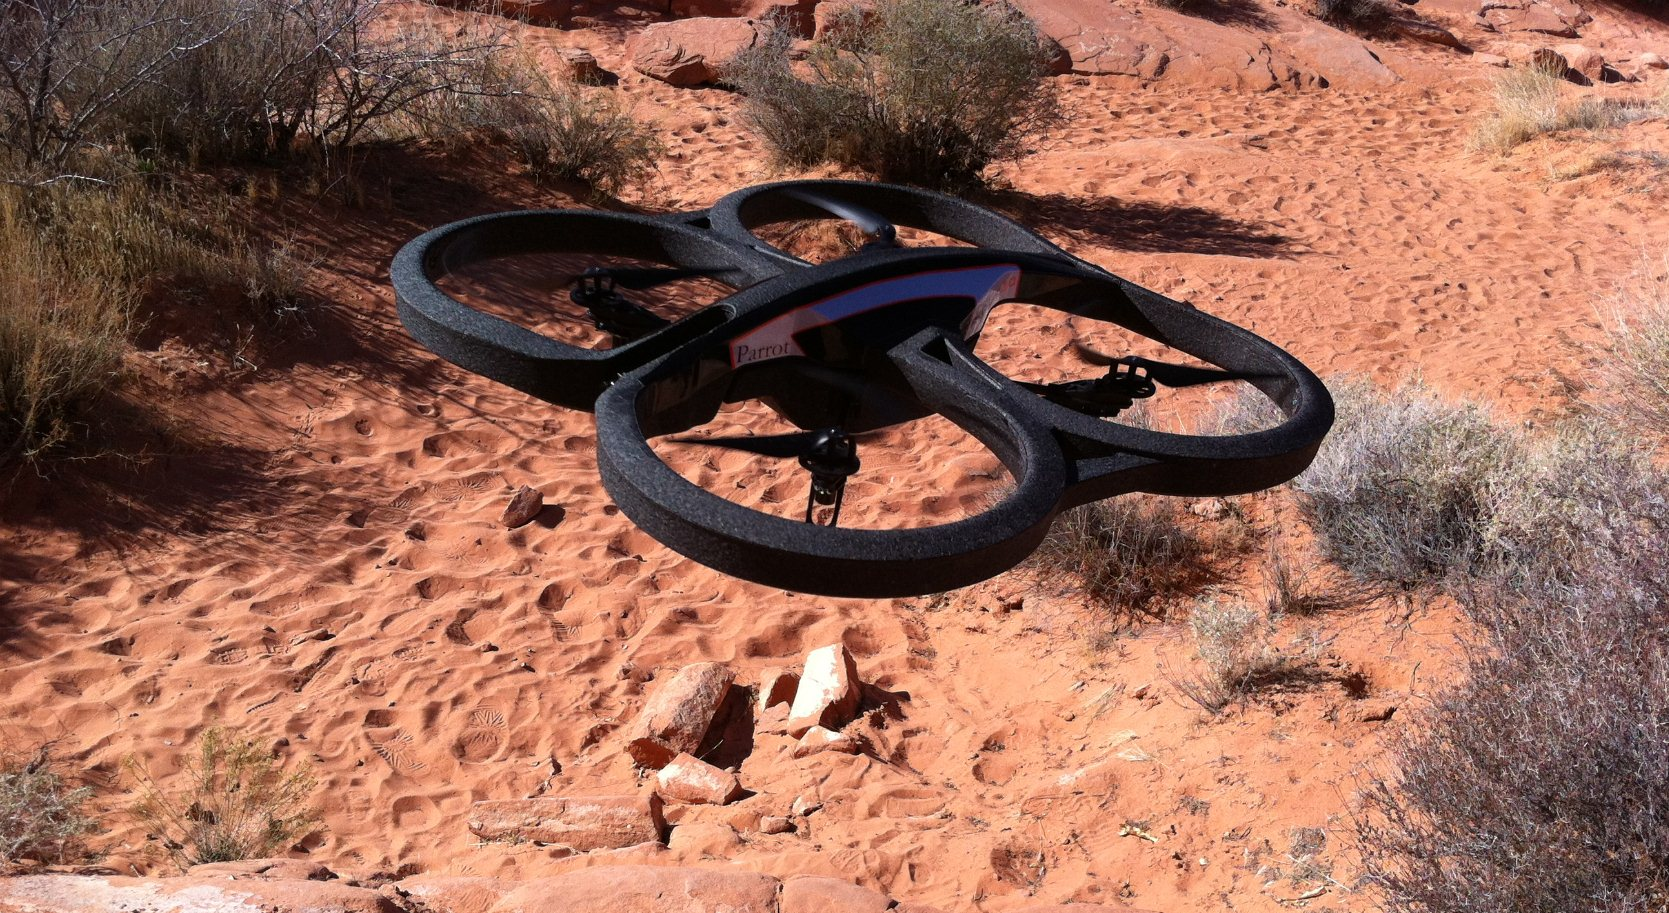
\includegraphics[height=8cm]{Title/parrotar}\\[2cm]
			% Title
			\HRule \\[0.4cm]
			{ \LARGE \bfseries Quadrotor Dynamics and Estimation\\[0.2cm]}\small ASEN 5044 :: Statistical Estimation of Dynamic Systems\\[0.4cm]
			\HRule \\[1cm]
			% Author and supervisor
				\begin{minipage}{0.4\textwidth}
					\begin{flushleft} \large
						\hspace*{-1em}\emph{Authors:}\\
						Zachary \textsc{Vogel}\\
					\end{flushleft}
				\end{minipage}
				\begin{minipage}{0.4\textwidth}
					\begin{flushright} \large
						\hspace{-2em}\emph{ } \\
						Aubrey \textsc{Harris}
					\end{flushright}
				\end{minipage}
				\vfill
				\vspace{.75cm}
			% Bottom of the page
				\begin{minipage}{0.4\textwidth}
					\begin{flushleft} 
						
\includegraphics[width=2cm]{Title/CUSeal.jpg}\\
					\end{flushleft}
				\end{minipage}
				\begin{minipage}{0.4\textwidth}
					\begin{flushright}
						
\includegraphics[width=1.75cm]{Title/CULogo.jpg}\\
					\end{flushright}
				\end{minipage}\\
			{\small 16 December 2016}\\
		\end{center}
	\end{titlepage}
\newpage

%%%%%%%%%%%%%%%%%%%% PRE-DOCUMENT CONTENTS %%%%%%%%%%%%%%%%%%%%%%
%Table of Contents
\setcounter{tocdepth}{2}
\setcounter{secnumdepth}{2}
\tableofcontents	
\newpage
\hypersetup{%
  colorlinks=true,% hyperlinks will be coloured
  linkcolor=blue,% hyperlink text will be green
}
%%%%%%%%%%%%%%%%%%%% FORMATTING NOTES %%%%%%%%%%%%%%%%%%%%%%
%%%%%%%%%%%%%%%% (Don't delete/uncomment) %%%%%%%%%%%%%%%%%%
%
%\begin{sect} %Custom environment for section
%\section{SECTION HEADING} %No content in sect environment
%\end{sect}
%   
%    SECTION CONTENT\\
%    \subsection{SUBSECTION HEADING}
%        SUBSECTION CONTENT\\
%        
%        \begin{subsubs} %Custom environment for subsubsection
%        \subsubsection{SUBSUBSECTION HEADING}
%            SUBSUBSECTION CONTENT\\
%        \end{subsubs}

%%%%%%%%%%%%%%%%%%%% DOCUMENT CONTENTS %%%%%%%%%%%%%%%%%%%%%%
\section{Introduction}{
This paper focuses on determining the estimation problem when centered on a quadrotor vehicle. We utilize various forms of the Kalman Filter and related techniques to explore the challenges of state estimation.  This assignment is in response to the final project for ASEN 5044 Statistical Estimate of Dynamic Systems at the University of Colorado, Boulder.
}
\section{Objective and Motivation}
The overarching goal of this project is to study the topic of estimation of system states. To do this, the report leverages computer simulations and a linearized model to gain an understanding of estimation and state prediction. This includes simulating several different forms of the Kalman filter utilized within a Luenberger Observer, simple tests of the effectiveness of said filters, as well as related concepts like pole placement. 

The motivation for studying the dynamics of a quadrotor system in respect to the objective is based upon their wide applicability in consumer products and their increased popularity in recent years.  The unique aspect of a quadrotor UAV is based upon the principle that it has six degrees of freedom but only four rotor actuators to provide control, making it nonlinear and an under-actuated system. The reason that this system makes for an excellent state estimation project is due to the chaotic nature of wind disturbances in real world applications of the problem as well as the wide range of sensors that can be used to determine the states of the system. 

%%Honestly tthis is mostly fluff and not really essential to the project.
%Unmanned aerial vehicles are aircraft that do not have a pilot and have existed in conceptual forms since World War I.  Sometimes more commonly referred to as “drones”, they have seen increased military implementation since the first Gulf War in the early 1990’s and Operation Enduring Freedom in the 2000’s in the form of the fixed wing Predator and Global Hawk UAVs; used for information, surveillance, and reconnaissance (ISR)\ref{fig:uav}.
%\begin{figure}[h!]
%    \centering
%    \begin{subfigure}[b]{0.4\textwidth}
%        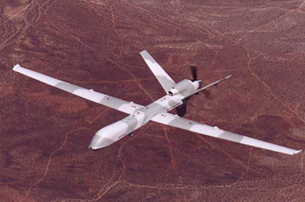
\includegraphics[width=\textwidth]{Images/uav}
%    \end{subfigure}
%    ~ %add desired spacing between images, e. g. ~, \quad, \qquad, \hfill etc. 
%      %(or a blank line to force the subfigure onto a new line)
%    \begin{subfigure}[b]{0.4\textwidth}
%        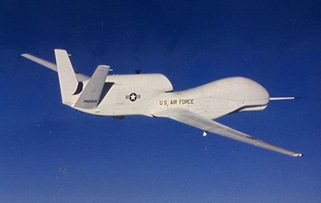
\includegraphics[width=\textwidth]{Images/uav2}
%    \end{subfigure}
%    \caption{USAF Predator and Global Hawk UAV}\label{fig:uav}
%\end{figure}
%Success in military applications led to increased use in civil and commercial markets such as NASA’s Earth science research division, law enforcement, border patrol, search and rescue, or even retailers such as Amazon investigating the potential for using UAVs to deliver goods to consumers.

\section{System Model}
\subsection{Multirotor Model}{
\begin{figure}[h!]
    \centering
    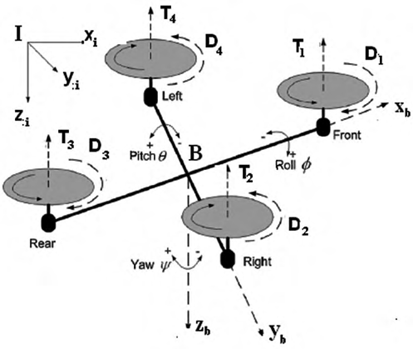
\includegraphics[width=0.6\textwidth]{Images/Quadrotor}
    \caption{Standard Quadrotor Model}\label{fig:Model}
\end{figure}
A quadrotor is comprised of four separate rotors, configured in a cross pattern with two rotors having counterclockwise flow while the other pair opposes with clockwise rotation.  The six degrees of freedom a quadrotor consist of the fore and aft motion (x-axis), lateral or side to side motion (y-axis), and the vertical or up and down motion (z-axis), as well as the pitch, roll, and yaw moments about those three axes.  For the purposes of this report we will assume the orientation of the quadrotor to be fixed similar to an aircraft flying straight and level so the 6 parameters for estimation will be the quadrotors position and change in position, ie $\pmb{x}=[x, dx, y, dy, z, dz]^T$.


%The quadrotor can change altitude, position, and orientation by changing the speed of each rotor depending on the desired maneuver. To change only the altitude the quadrotor would increase the speed of all four rotors equally for takeoff or decrease the speed of all four rotors equally to land.  


%To alter the fore and aft motion the quadrotor would increase the speed of the aft rotor while decreasing the forward rotor while maintain the speed of the lateral rotors which would result in a decrease in pitch and forward motion along the x-axis.  An opposite increase in speed from the forward rotor and a decrease in speed from the aft rotor would result in a positive change and pitch and subsequent backwards motion along the x-axis.  The same maneuvers could be performed by the lateral rotors to execute a left or right roll and produce lateral motion. 

%A yaw is execute by increasing the rotation speed of a pair of rotors while decreasing the other pair’s speed.  The difference in net torque produces a yaw effect and the direction of the yawing motion depends on whether the speed of the clockwise or counterclockwise rotor pair is increased.  Figure \ref{fig:move} depicts these maneuvers with a thicker arrow illustration an increase in rotor speed.


%above is overly wordy. 1 paragraph is fine

\begin{equation}
\begin{split}
Fx= \delta(T3-T1)
\\
Fy= \delta(T4-T2)
\\
Fz= \gamma(T4+T3+T2+T1)
\end{split}
\label{inputs}
\end{equation}

Based on equation and figure \ref{fig:Model} we can see how the vehicle moves in reference to its relative force in each axis. The difference in torque between the fore and aft rotors, labeled $T_1$ and $T_3$ yields movements along the x-axis, difference in torque between the lateral rotors, labeled $T_2$ and $T_4$, creates side to side motion and the sum of torques between all the motors creates vertical movement. This will be used to determine our desired inputs in section 3.5. The resulting forces in the $x,y$ and $z$ directions are shown in equation \ref{inputs}.

%As previously mentioned, if we assume a symmetric vehicle with four identical rotors, where one pair spins in one direction and the other pair spins in the opposite direction, the quadrotor can be linearized in respect to our states, $\pmb{x}=[x, dx, y, dy, z, dz]^T$.
%This model consists of the x, y, and z positions in a fixed coordinate frame along with their respective velocities. The control or input vector is represented by $\pmb{u}=[T_1, T_2, T_3, T_4]^T$. In this model $T_1$ through $T_4$ represents the thrust inputs for each of the four rotors.  The resulting force in the x, y, and z directions are represented by the equations in 1.
\begin{equation}\begin{split}
 \dot{\pmb{x}}=A\pmb{x}+B\pmb{u}=\begin{bmatrix}0&1&0&0&0&0\\
    0&-.0104&0&0&0&0\\
    0&0&0&1&0&0\\
    0&0&0&-.0104&0&0\\
    0&0&0&0&0&1\\
    0&0&0&0&0&-.0208\end{bmatrix}\begin{bmatrix}x\\dx\\y\\dy\\z\\dz\end{bmatrix}
  +\\
  \begin{bmatrix}0&0&0&0\\
   -.04167&0&.04167&0\\
   0&0&0&0\\
   0&-.04167&0&.04167\\
   0&0&0&0\\
   .4&.4&.4&.4\end{bmatrix}\begin{bmatrix}T_1\\T_2\\T_3\\T_4\end{bmatrix}
\end{split}\label{model}\end{equation}


%Fz is the resulting upwards force of the four rotors which is responsible for the
%change in altitude of the quadrotor and its rate of change. Fy is the difference in thrust between rotors 2 and 4 which is responsible for the roll rotation, lateral motion, and its rate of change. Fx, conversely, represents the difference in thrust between rotors 1 and 3.  This difference generates a change in pitch rotation, forward and aft motion, and its respective rate of change. A fourth parameter is the difference between counter rotating rotor pairs would generate a yaw moment causing the vehicle to turn, however for the purposes of this project we will assume that the quadrotor is in a fixed orientation about the x-axis.
{
}


Given that $F_x$ is the force in the x direction, $F_y$ is the force in the y direction and $F_z$ in the z direction. With these forces, we are able to control the position of the vehicle. Typically there would normally be another 6 states governing angular orientation and velocity, but these are ignored for the purposes of this project. Having these inputs, we can now right a state equation based on the linearized state relationships given in the project outline and illustrated in equation \ref{model}.


\newpage{}

%\pmb{y}=C\pmb{x}+D\pmb{u}=\begin{bmatrix}1&0&0&0&0&0\\
%0&0&1&0&0&0\\
%0&0&0&0&1&0\end{bmatrix}x+\pmb{0}
}
\subsection{Process Noise Model}{
    In the case of a multirotor, the process noise is largely focused on wind based disturbances. Here we will consider these as being random forces that impart an acceleration onto the quadrotor. We also acknowledge that winds along the z-axis are likely less powerful assuming the z-axis is perpendicular to the Earth's surface. Thus our new state model is shown in equation \ref{process noise} where $\omega\sim\mathcal{N}(0,\tilde{Q})$.
    \begin{equation}\label{process noise}\begin{split}
        \dot{\pmb{x}}=A\pmb{x}+B\pmb{u}+\Gamma\omega\\
        \Gamma=\begin{bmatrix}
            0&0&0\\
            1&0&0\\
            0&0&0\\
            0&1&0\\
            0&0&0\\
            0&0&1
            \end{bmatrix}\quad
        \tilde{Q}=\begin{bmatrix}
        0.02&0.005&0.005\\
        0.005&0.02&0.002\\
        0.002&0.002&0.005\end{bmatrix}
        \end{split}\end{equation}
    The chosen $\tilde{Q}$ matrix was based of off intuition. The magnitude can't be much bigger than the magnitude of the coefficients in the $A$ and $B$ matrices or the noise term will dominate. One also has to note that the z-axis will likely be close to perpendicular to the ground. Wind forces in the z axis when it is perpendicular to the ground will likely be lower than in the x and y axis. The $\tilde{Q}$ matrix is used to determine the process noise matrix $Q$ via Van Loans Method, and is in units of $m/s^2$.
}
\subsection{Measurements}{
    The main sensor model we used for this project was simply a measurement of the vehicle positions in free space, noted by the C matrix in equation \ref{output}. We also considered measurements of velocity and strictly the x and y states. The state to output relations for these can be seen in equation \ref{output1}, where $C_1$ is measuring velocities and $C_2$ is measuring only two positions. It's important to briefly note that the input does not directly force the output and thus the matrix that directly relates input to output is filled with zeros. Other than that we must consider the measurement noise of our system. An article was found which gave the discrete time measurement noise intensity matrix. Thus we skipped straight to that value. Our final measurement model is shown in equation \ref{output}.
    \begin{equation}\label{output}
        \pmb{y}=C\pmb{x}+D\pmb{u}+v=
        \begin{bmatrix}
        1&0&0&0&0&0\\
        0&0&1&0&0&0\\
        0&0&0&0&1&0
        \end{bmatrix}\pmb{x}+\pmb{0}\pmb{u}+v       
    \end{equation}
    \begin{equation}\label{output1}
        C_1=\begin{bmatrix}0&1&0&0&0&0\\0&0&0&1&0&0\\0&0&0&0&0&1\end{bmatrix}\qquad
        C_2=\begin{bmatrix}1&0&0&0&0&0\\0&0&1&0&0&0\end{bmatrix}
    \end{equation}
}
\subsection{Discretization}{
    To determine the sampling rate, we first found the eigenvalues of our A matrix. This gives eig($A$)=
    $[0,-0.0104,0,-0.0104,0,-0.0208]$.  Here we focus on $\lambda=-0.0208$.  This is because this specific pole will respond faster than the other poles.  Thus, if we can keep track of it we will be able to keep track of the remaining poles in theory.  This value could also be described as half the Nyquist frequency.  Generally, we want to sample at a minimum of 10 times the Nyquist frequency.  Thus our sampling frequency needs to be at least $0.4$ rad/s. This equates to a period of 15 seconds.  This seemed way too high so instead our team elected to use a sampling rate of $0.1$ seconds due to the feedback gain matrix given in the project proposal being sampled at that rate.
    \begin{equation}\label{disc_model}
    \begin{split}
        \pmb{x}_{k+1}=F\pmb{x}_k+G\pmb{u}(k)+w_k\qquad w_k\approx\mathcal{N}(0,Q)\\
        y_k=H\pmb{x}_k+v_k\qquad v_k\approx\mathcal{N}(0,R)
    \end{split}
    \end{equation}
    We then discretized the system using the c2d command in MATLAB to determine the correct matrices relating to state updates, inputs to state updates, and states to outputs. To find the discrete time process noise intensity matrix, we used Van Loan's method. The measurement noise intensity was taken from a paper on the topic. The generic model written out in equation \ref{disc_model} is filled with the matrices in \ref{disc_mat}.
    \begin{equation}\label{disc_mat}
    \begin{split}
        F=\begin{bmatrix}
        1.0000  &  0.0999  &   0    &     0      &   0    &     0\\
        0    &0.9990     &    0    &     0      &   0   &      0\\
         0    &     0    &1.0000   & 0.0999     &    0  &       0\\
         0     &    0    &     0   & 0.9990     &    0  &       0\\
         0      &   0    &     0   &      0    &1.0000  &  0.0999\\
         0       &  0    &     0    &     0 &    0  &  0.9979
         \end{bmatrix}
         \\
         G=\begin{bmatrix}
            -0.0002     &    0   & 0.0002     &    0\\
              -0.0042  &       0  &  0.0042   &    0\\
             0  & -0.0002        & 0&    0.0002\\
             0  & -0.0042        & 0 &   0.0042\\
            0.0020   & 0.0020    &0.0020  &  0.0020\\
            0.0400   & 0.0400    &0.0400  &  0.0400
            \end{bmatrix}
            \\
            H=\begin{bmatrix}
        1&0&0&0&0&0\\
        0&0&1&0&0&0\\
        0&0&0&0&1&0
        \end{bmatrix}
            \\
        Q=\begin{bmatrix}
            0.0000   & 0.0001&    0.0000  &  0.0000&    0.0000  &  0.0000\\
            0.0001   & 0.0020&    0.0000  &  0.0005 &   0.0000  &  0.0002\\
            0.0000   & 0.0000&    0.0000  &  0.0001  &  0.0000  &  0.0000\\
            0.0000   & 0.0005&    0.0001  &  0.0020   & 0.0000  &  0.0002\\
            0.0000   & 0.0000&    0.0000  &  0.0000    &0.0000  &  0.0000\\
            0.0000   & 0.0002&    0.0000  &  0.0002    &0.0000  &  0.0005
        \end{bmatrix}\\
                R=diag([0.0933,0.0885,0.2450])
    \end{split}
    \end{equation}
}

\subsection{Input Characterization}


\begin{figure}[h!]
    \centering
    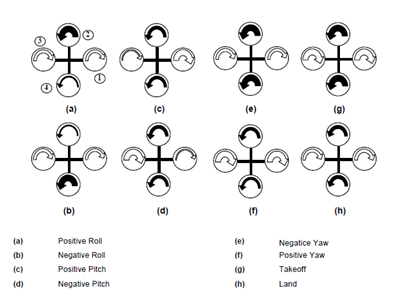
\includegraphics[width=0.8\textwidth]{Images/quadrotor2}
    \caption{Basic quadrotor motions}\label{fig:quadmotions}
\end{figure}
In figure \ref{fig:quadmotions} the basic commands to generate a specific type of movement are seen. In respect to our model and problem, where we aren't considering orientation, we are not concerned with yaw. Thus we created an input that produced all 6 other types of motion created here. This meant we gave an input to give pure upward force, downward force, positive roll, negative roll, positive pitch, and negative pitch. This results in a force in both the positive and negative of each axis. Zach realized very late Wednesday night that Professor Ahmed had asked for strictly a negative feedback control law using the matrix $T$ from the proposal. It can be seen with less significant figures in equation \ref{Tmat}. At this point he had already created the input as described above and was using that as well as the feedback control law in the form $G*(u-T*x)$.
\begin{equation}\label{Tmat}
    T=\begin{bmatrix}
    -.9798& -4.825& -.2308& -.6122& .6905& 1.223\\
    6.8979e-15& 1.486e-14& -.3775& -.9385& .7149& 1.287\\
    .9799& 4.825& -.2308& -.6122& .6905& 1.223\\
    -2.500e-15& -1.303e-14& 1.235& 2.650& .4464& .5857
    \end{bmatrix}
\end{equation}

\section{System Analysis}{

\subsection{Observability}{
    A key concept relating to the use of Kalman filtering is the concept of observability. This determines if it is possible to "back out" the states of a system from the set of measurements one actually takes. For linear time-invariant systems, the observability matrix guarantees observability of a system if the rank of said observability matrix is equivalent to the number of states in the system. This matrix is formed as in equation \ref{observability} where n is the number of states.
    \begin{equation}\label{observability}
        \mathfrak{O}=\begin{bmatrix}H\\HF\\HF^2\\\vdots\\HF^{n-1}\end{bmatrix}
    \end{equation}
    This calculation was performed for the $F$ and $H$ matrices of the system. This resulted in an observability matrix with rank 6. Thinking about this further, it makes perfect sense. With the measurements of the position at every time step one can also estimate the derivative of the terms. To explore this further, the matrices in equation \ref{output1} were used to do another observability analysis. The first matrix in that equation, noted $C_1$, produced an observability matrix with rank 3. This makes sense because it only measured the velocities. From velocities, one can derive the displacement, but never the actual position without an initial measurement of position. The matrix $C_2$ produces an observability matrix with a rank of 4. This gave the position and velocity of the two measured terms, but without any correlating factors between the positions in the state equation, backing out the other position and velocity is impossible.
}
\subsection{Initialization}{
To initialize our system we assumed an initial mean value of $[1, 0, 1, 0, 1,0]$ and an initial covariance equal to the identity matrix.  To predict each of the states forward in time we iterate our simulation at each time step (.1 seconds) over our duration (40 seconds) to determine the mean and covariance values at each time step, equations \ref{mean} and \ref{covariance}.

\begin{equation}\label{mean}\centering
    \mu(k+1)=F*\mu(k)+G*u(k)
\end{equation}
\begin{equation}\label{covariance}\centering
    P(k+1)=F*P(k)*F^T+Q
\end{equation}

Other than simply giving the true state value for our system as the initialization value. Batch least squares was also derived and attempted for extra credit. This involved taking the derivative of the $J(\theta)$ function as described in slides 26. The resulting equations are given in equation \ref{bls}. Any equation not specifically stated here can be taken from lecture slides 26 for the class. Most of the ones not listed are large block matrices. Unfortunately, these equations failed to find the correct initial estimate for the system. Thus, there was no point in continuing forward and determining the covariance estimates at each time step. The initial guess for $x_0$ was
\begin{equation}\label{bls}
\begin{split}
    \bar{A}_x=-(\bar{H}^T\bar{R}^{-1}\bar{H})^{-1}\bar{H}^T\bar{R}^{-1}\\
    \bar{A}_w=(\bar{C}^T\bar{R}^{-1}\bar{C}+\bar{Q}^{-1})^{-1}\bar{C}^T\bar{R}^{-1}\\
    \bar{L}_x=\bar{A}_x(\bar{y}-\bar{G}\bar{u})\quad \bar{M}_x=\bar{A}_x\bar{C}\\
    \bar{L}_w=\bar{A}_w(\bar{y}-\bar{G}\bar{u})\quad \bar{M}_w=\bar{A}_w\bar{H}\\
    xbls_0=(I-\bar{M}_x\bar{M}_w)^{-1}(\bar{M}_x\bar{L}_w+\bar{L}_x)\quad wbls=(I-\bar{M}_w\bar{M}_x)^{-1}(\bar{M}_w\bar{L}_x+\bar{L}_w)
\end{split}
\end{equation}
}



\subsection{Monte Carlo}{
\begin{figure}[h!]
    \centering
    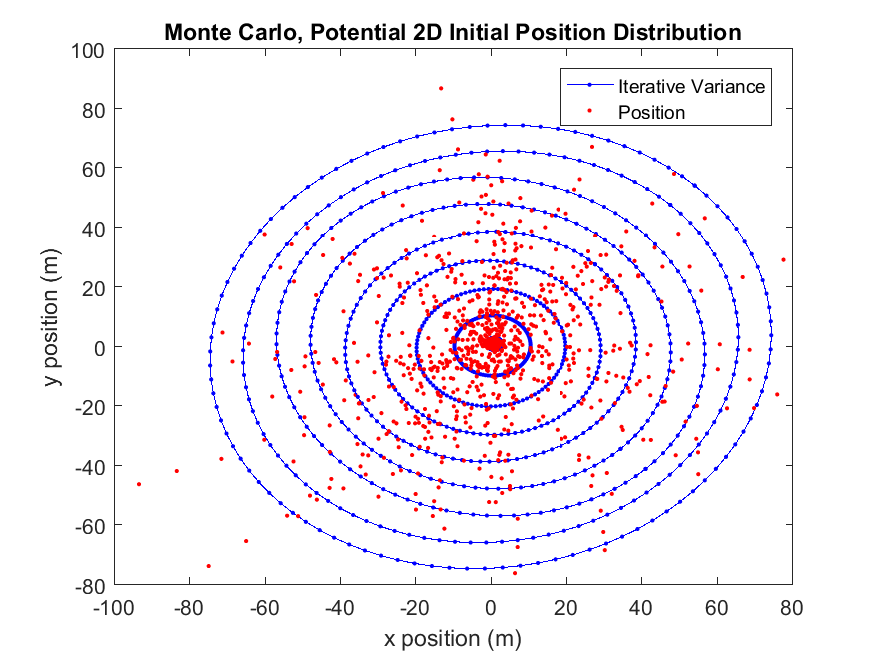
\includegraphics[width=0.8\textwidth]{Images/MC.png}
    \caption{Monte Carlo Covariance Simulation}\label{fig:monte_carlo}
\end{figure}
Monte Carlo simulations are ran to predict the system by plotting sample points based on a Gaussian distribution of the initial mean and covariance iterated over time as seen in figures \ref{fig:monte_carlo}, \ref{Mcxy} and \ref{Mcz}. It's easy to see that the velocity of the quadrotor in the x and y directions has a constant error bound, the bound of the velocity in the z-axis is decreasing and the position bounds in all three axis are increasing with time. This also illustrates the necessity of a feedback control law as we simply can't minimize error to a steady state value without it.

\begin{figure}[h!]
    \centering
    \begin{subfigure}[b]{0.49\textwidth}
        \centering
        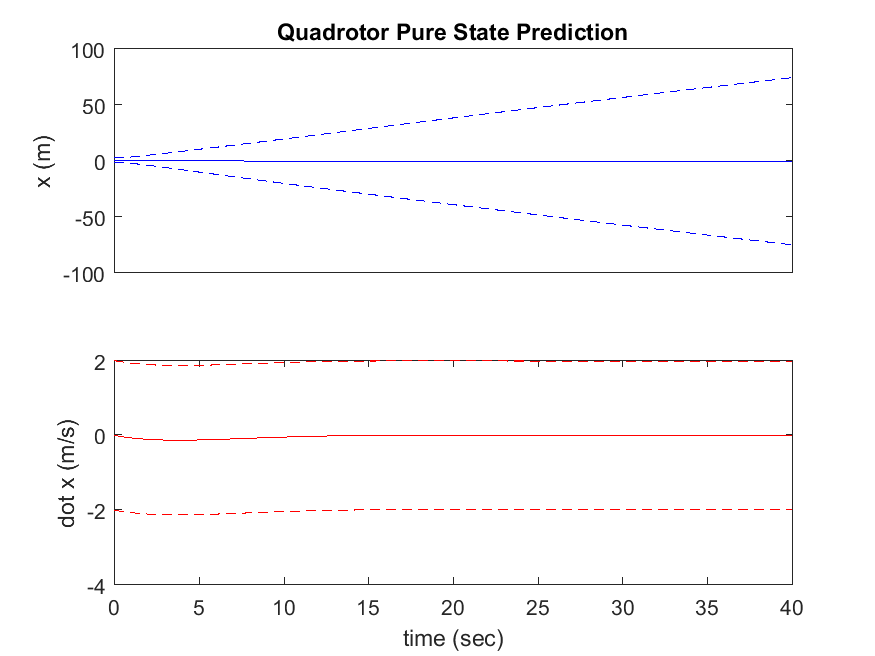
\includegraphics[width=\textwidth]{Images/MCx.png}
    \end{subfigure}
    \begin{subfigure}[b]{0.49\textwidth}
        \centering
        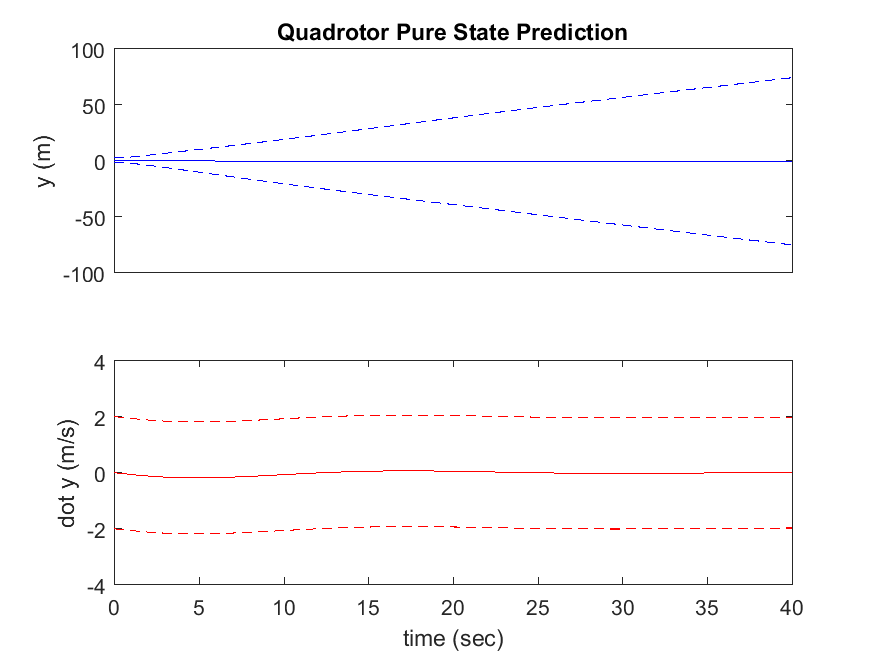
\includegraphics[width=\textwidth]{Images/MCy.png}
    \end{subfigure}
     \caption{Monte Carlo state prediction for x and y positions and their derivatives}
    \label{Mcxy}   
\end{figure}


\begin{figure}[h!]
        \centering
        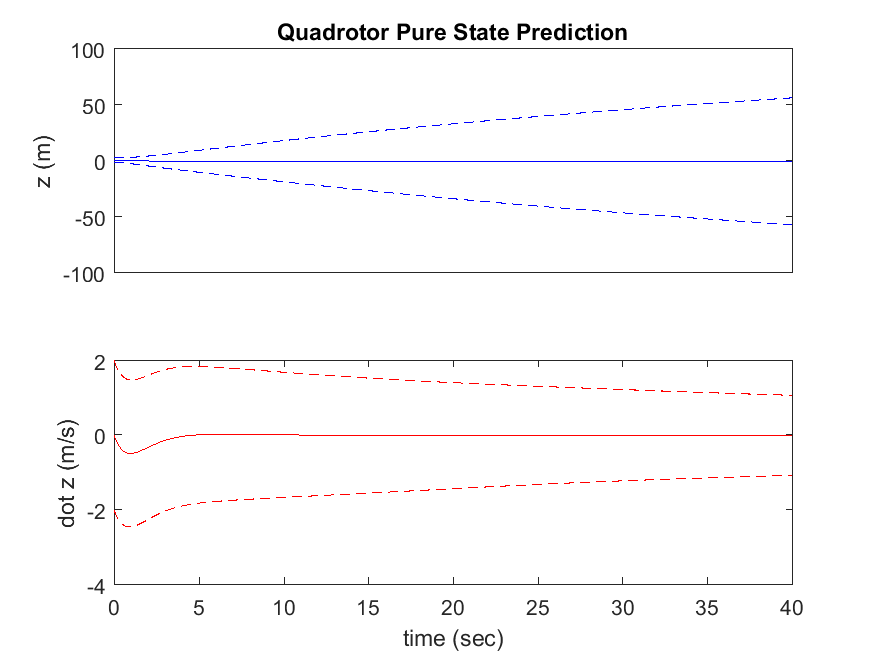
\includegraphics[width=0.5\textwidth]{Images/MCz.png}
    \caption{Monte Carlo state prediction for z position and its derivative}
    \label{Mcz}
\end{figure}
}
}
\newpage
\section{Simulation}{
\subsection{Kalman Filter}{
\begin{figure}[h!]
    \centering
    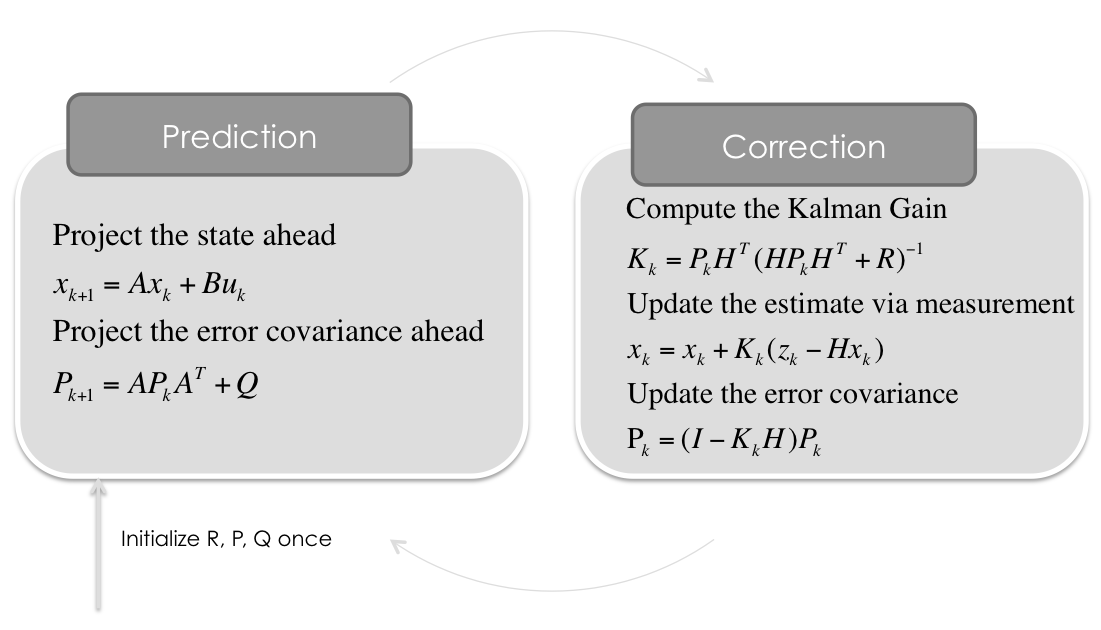
\includegraphics[width=0.6\textwidth,clip=true,trim={0cm 0 0cm 1cm}]{Images/Kalman-Filter-Step}
    \caption{Kalman Filter with a Luenberger Observer}\label{fig:Kal_filter_diagram}
\end{figure}
This project's analysis heavily leveraged the Kalman Filter which is an estimation tool for any continuously changing, dynamic system with unknown information such as process noise.  The Kalman Filter is a powerful tool for calculating a Luenberger Observer gain. It requires little memory because it stores the previous time step's estimated mean and covariance matrix as well as the linearized system model. The key components of a Kalman filter based observer are the prediction, which attempts to find the system states and covariance matrix with strictly the system model. Then a Kalman filter gain is calculated and used to weight the error between estimated system state and measurements of the system state. It is also used to update the covariance. This can be seen in figure \ref{fig:Kal_filter_diagram}.

\begin{figure}[h!]
    \centering
    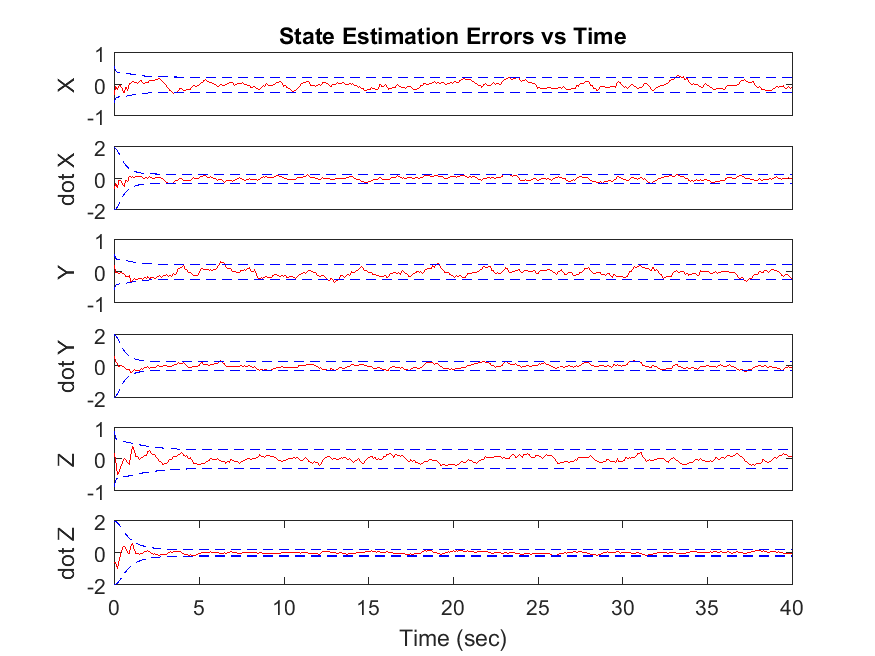
\includegraphics[width=0.8\textwidth,clip=true,trim={0cm 0 0cm 0}]{Images/KF.png}
    \caption{Quadrotor Kalman Filter Results}
    \label{fig:Kalman_filter_res}
\end{figure}


Figure \ref{fig:Kalman_filter_res} illustrates the results of the traditional Kalman or covariance filter for each of the six states during the 40 second observation window where the filter is predicting the state position and velocity with a two sigma covariance boundary. Figure \ref{fig:Kalman_filter_err} illustrates the same expected errors for each state on a combined graph.

\begin{figure}[h!]
    \centering
    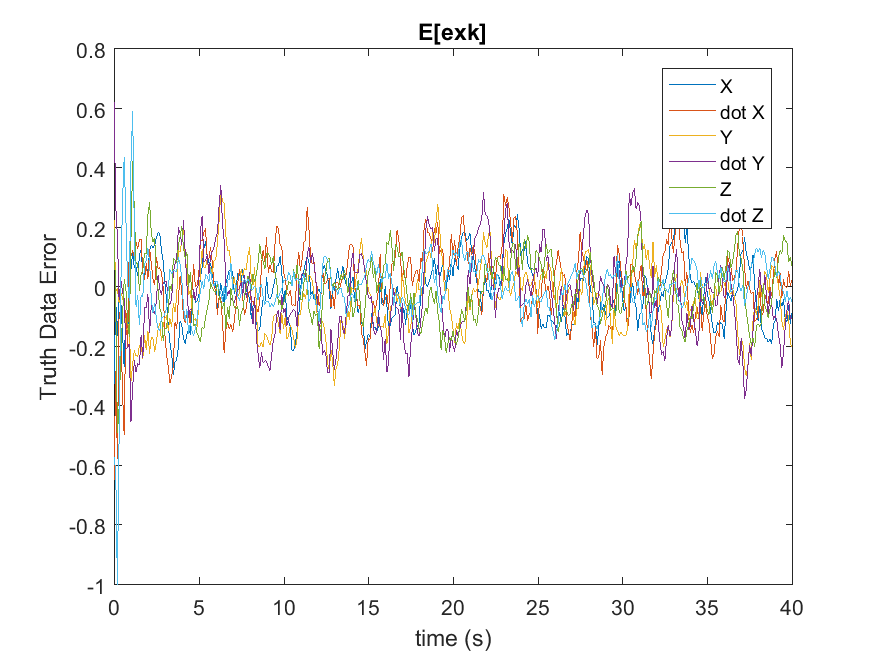
\includegraphics[width=0.6\textwidth]{Images/errors.png}
    \caption{Quadrotor Error History}
    \label{fig:Kalman_filter_err}
\end{figure}


The vanilla Kalman Filter does a very good job of estimating the states of the system. The 2 $\sigma$ bound converges very quickly to a reasonable level of less that 1 for all system states. The state error stays within these bounds for the majority of the simulation run.



}
\subsection{Information Filter}{
This section was completed by Aubrey Harris.

\begin{figure}[h!]
   \centering
    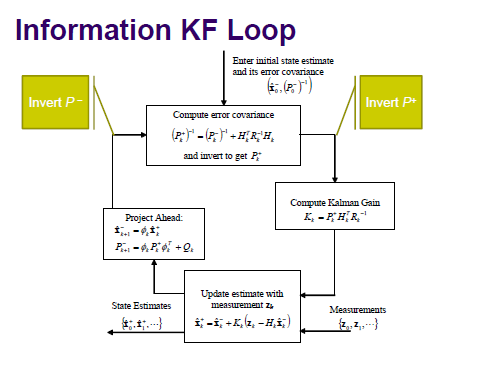
\includegraphics[width=0.7\textwidth,clip=true,trim={0cm 0.7cm 0cm 0}]{Images/Information}
    \caption{Information Filter}\label{fig:Info_filt}
\end{figure}

The Information Filter (IF) is an alternative to the Kalman Filter where the information matrix (Ik) is the inverse of the error covariance matrix (Pk).  The Information Filter is a useful estimation tool when little is known about the dynamic systems such that the initial error covariance matrix is very large where the traditional Kalman Filter would struggle to initialize.  The information filter requires an additional inversion loop with the apriori and aposterior covariance matrices (Figure \ref{fig:Info_filt}) and requires the information matrix to be fully observable.

\begin{figure}[h!]
    \centering
    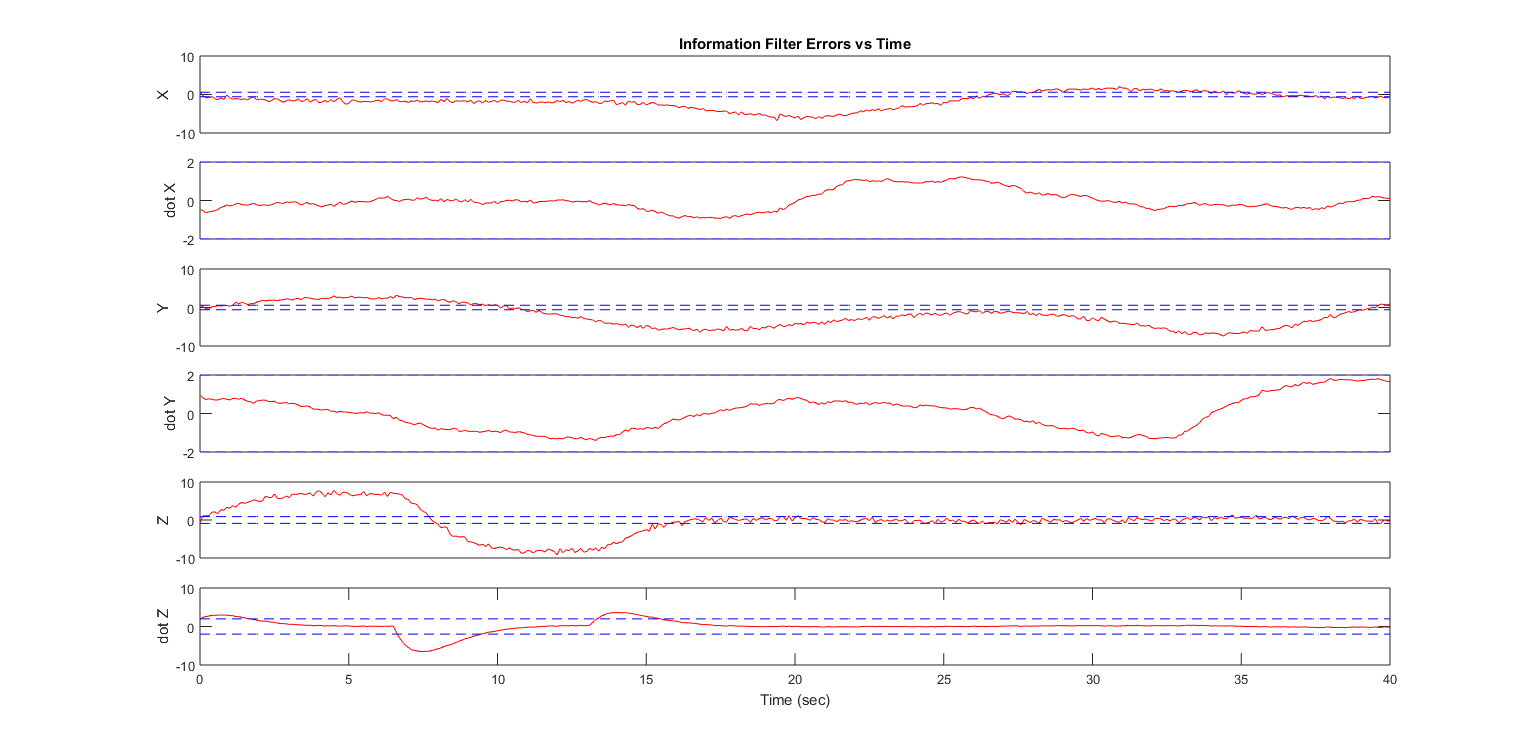
\includegraphics[width=\textwidth,clip=true,trim={0cm 0 0cm 0}]{Images/IF2.png}
    \caption{Quadrotor Information Filter}\label{fig:Info_filter_Results}
\end{figure}

The numerical values for the Information and Kalman Filters should be the same once the mean and covariance matrices are properly recovered.  The Information Filter is most useful when the system's states are fully understood or the error matrix is large, however due to the added requirement to invert the error covariance matrix into the information matrix and subsequently recover the mean and covariance matrices the Information Filter is rarely more efficient than the traditional Kalman Filter based on computational requirements.  Additionally our information filter does not mirror the values from our Kalman Filter results most likely due to numeric errors in coding (Figure \ref{fig:Info_filter_Results}).  Two different attempts were made at reproducing the information filter (class lecture and research sources) however neither produced precise results, most likely due to operator error.

}

\subsection{Square Root Filter}{


In a similar vein, a square root filter can be implemented in place of a traditional Kalman Filter and was attempted for extra credit.  The benefits of square root filters showcase themselves when process noise is small.  In events such as these roundoff errors can occur, turning eigenvalues negative and making the overall process noise matrix indefinite versus positive semi-definite.  Utilizing Cholesky factorization or triangular matrix square root we may be able to reference a more robust form of the Kalman filter as seen in figure \ref{fig:SRKF}, where ($P=S*S^T$).

\begin{figure}[h!]
    \centering
    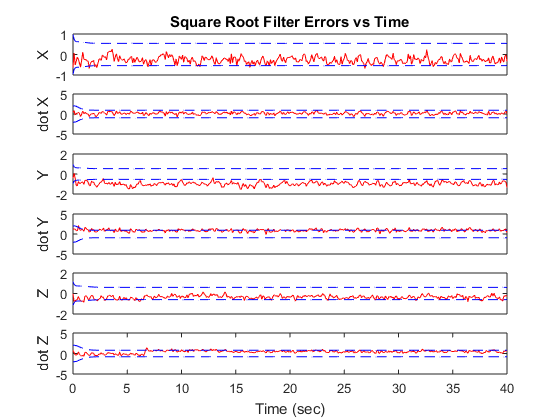
\includegraphics[width=\textwidth,clip=true,trim={0cm 0 0cm 0}]{Images/SRKF4.png}
    \caption{Quadrotor Square Root Filter}\label{fig:SRKF}
\end{figure}

As can be seen from the results of the square root filter, some amount of offset error seemed to occur. If the error was displaced by this offset value the signals would have been within reasonable 2 $\sigma$ bounds, but existed almost entirely outside of these regions. This leads us to believe that the vanilla Kalman Filter was the best tool. This could be attributed to that fact that our system has been properly linearized to a modest scenario (ie-hover or fixed motion along a single axes), therefore the model matches the real system fairly accurately and alternative methods might not be optimal due to increased computing requirements, processing time, and potential for coding errors.

}

\subsection{Pole Placement Observer}{
This section was completed by Zachary Vogel.
\begin{figure}[h!]
    \centering
    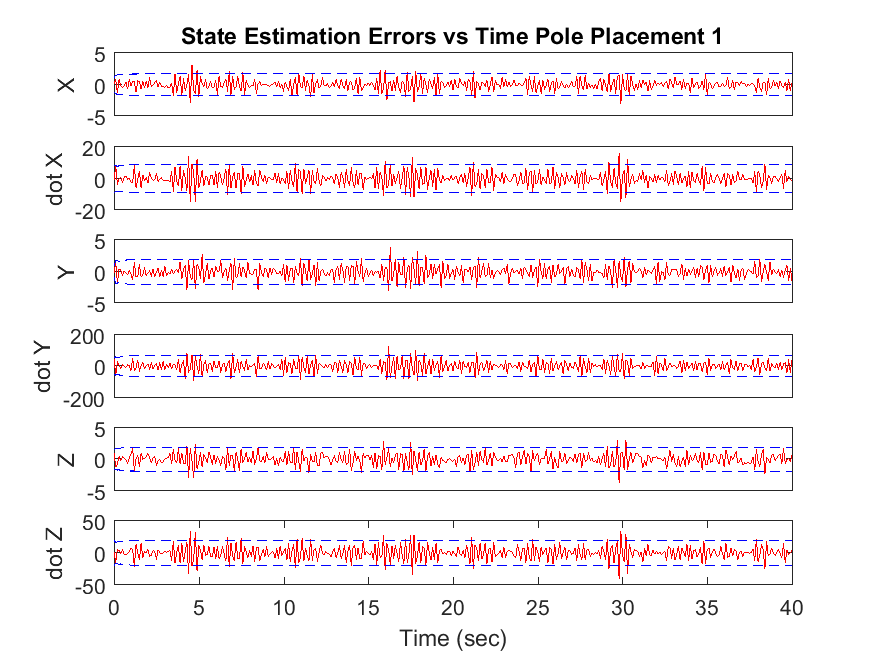
\includegraphics[width=0.8\textwidth,clip=true,trim={0cm 0 0cm 0}]{Images/pole1}
    \caption{Pole placement results 1 with $a=0.9$}\label{fig:pole1}
\end{figure}

Pole placement is the methodology were one uses a specific feedback gain in the Luenberger Observer as opposed to a time varying one as is the case for the Kalman filter. The advantage of the lower amount of calculations required, and that the poles of the observer are placed exactly where the the designer decided they should be. In this section, 3 trials were simulated over the standard time period. Poles were placed at $\lambda=a*[-0.707\pm 0.707i, 1,-0.3536\pm 0.3536i,0.5]$ with $a$ equal to $0.9$, $0.5$ and $0.2$.

The pole placement was done utilizing the place command, and did successfully place the poles at the desired locations. We also examined the location of the poles based on the final Kalman Filter gain for the vanilla Kalman Filter in order to compare to what is essentially the steady state gain. This gain placed the poles at $\lambda_{K}=[0.9090 \pm 0.0831i, 0.9200 \pm 0.0739i, 0.9533 \pm 0.0445i]$. Noting that there were significantly smaller imaginary parts to these poles, as well as their proximity much closer to the marginal stability point of $1$ in the discrete plane explains why the graphs in \ref{fig:pole1}, \ref{fig:pole2}, and \ref{fig:pole3} fail to get accurate state measurements.

The high imaginary values on the placed poles correspond to extra oscillations in the estimated values. The close proximity to the origin also means that higher gains are found in the placed pole gain matrices as compared to the Kalman filter gains. That means that errors in measurement are reacted to very quickly and in this case too much so. Small disturbances due to the simulated noise result in rapid state value changes.
\begin{figure}[h!]
    \centering
    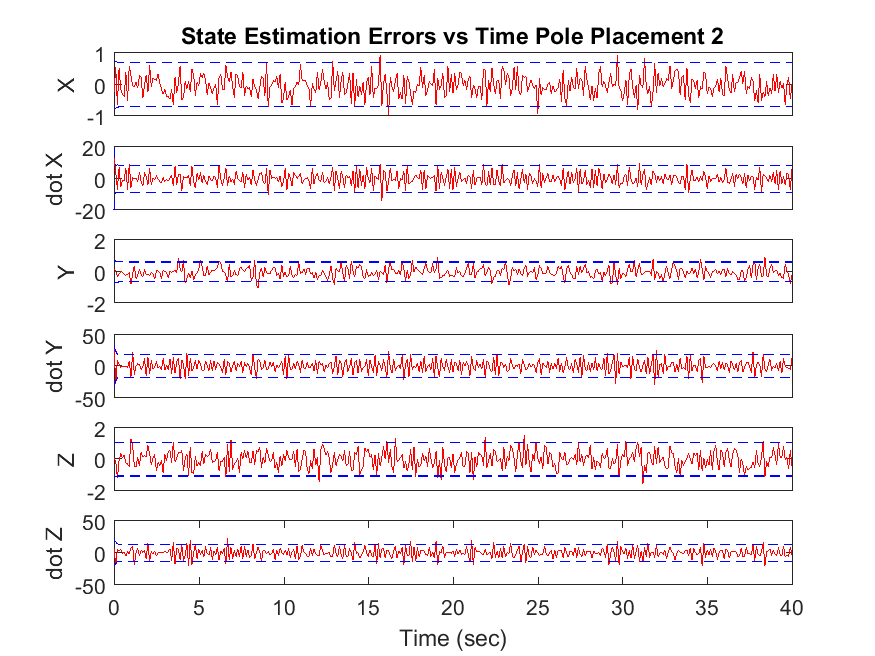
\includegraphics[width=0.8\textwidth,clip=true,trim={0cm 0 0cm 0}]{Images/pole2}
    \caption{Pole placement results 2 with $a=0.5$}\label{fig:pole2}
\end{figure}

\begin{figure}[h!]
    \centering
    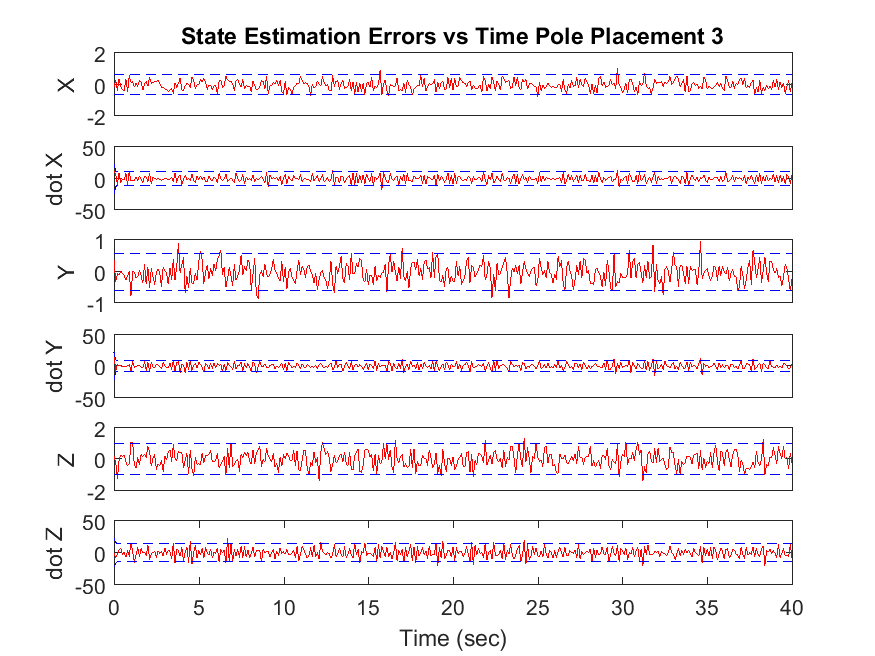
\includegraphics[width=0.8\textwidth,clip=true,trim={0cm 0 0cm 0}]{Images/pole3}
    \caption{Pole placement results 3 with $a=0.2$}\label{fig:pole3}
\end{figure}

}
}
\pagebreak
\section{Verification}{

\subsection{NEES and NIS Chi-Square Tests}{
\begin{figure}[h!]
    \begin{subfigure}[b]{0.49\textwidth}
        \centering
        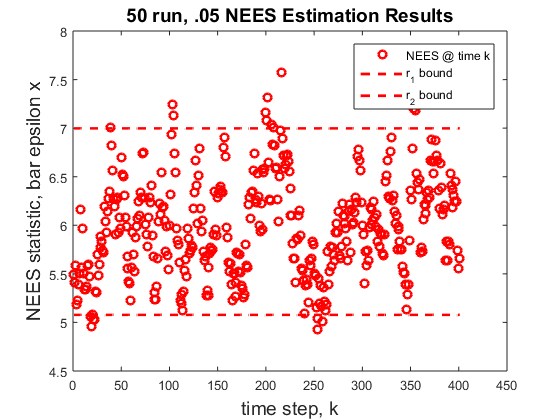
\includegraphics[width=\textwidth]{Images/50NEES.png}
    \end{subfigure}
    \begin{subfigure}[b]{0.49\textwidth}
        \centering
        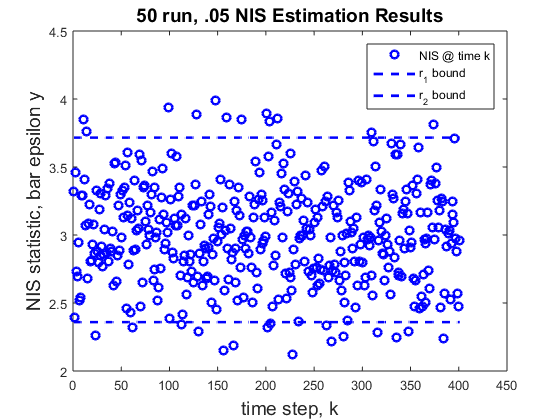
\includegraphics[width=\textwidth]{Images/50NIS.png}
    \end{subfigure}
    \caption{NEES and NIS simulation 1}
    \label{nissim1}
\end{figure}
The normalized estimated error square (NEES) and normalized innovation squared (NIS) tests are performed to determine whether or not the Kalman Filter simulation is consistent with the true model.  To run a chi-squared test a number of Monte Carlo simulations, or runs (N) need to be executed with a pre-determined level of significance (alpha) to prove consistency.  The generally accepted value for alpha is less than or equal to 0.05.


\begin{figure}[h!]
    \begin{subfigure}[b]{0.49\textwidth}
        \centering
        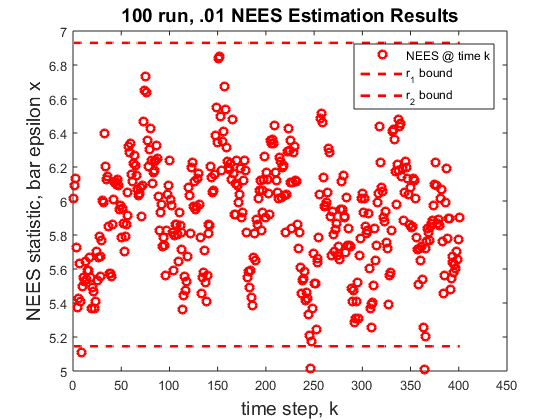
\includegraphics[width=\textwidth]{Images/100NEES.png}
    \end{subfigure}
    \begin{subfigure}[b]{0.49\textwidth}
        \centering
        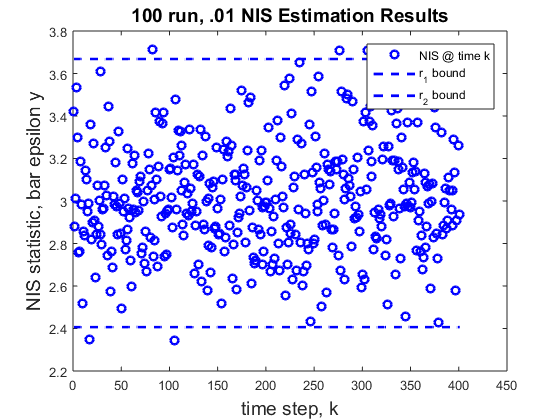
\includegraphics[width=\textwidth]{Images/100NIS.png}
    \end{subfigure}
    \caption{NEES and NIS simulation 2}
    \label{nissim2}
\end{figure}

Starting with the general accepted level of significance we can prove that our model is consistent if 95 percent of our data points fall within the boundary limits (2 sigma).  As the tolerances for outlaying data becomes more restrictive, the total number of runs needs to be increased to account for these reduced error bounds. 

\begin{figure}[h!]
    \begin{subfigure}[b]{0.49\textwidth}
        \centering
        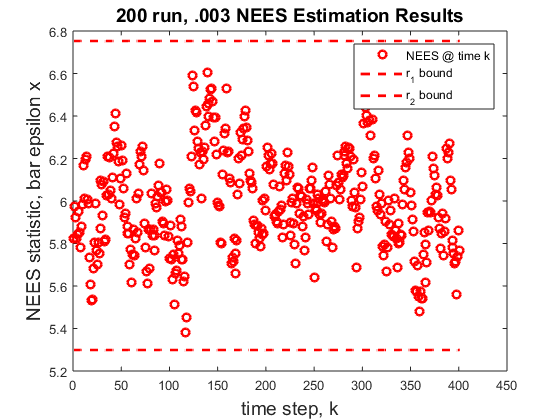
\includegraphics[width=\textwidth]{Images/200NEES.png}
    \end{subfigure}
    \begin{subfigure}[b]{0.49\textwidth}
        \centering
        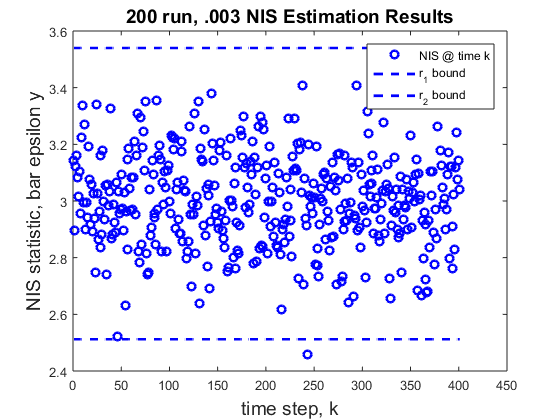
\includegraphics[width=\textwidth]{Images/200NIS.png}
    \end{subfigure}
    \caption{NEES and NIS simulation 3}
    \label{nissim3}
\end{figure}

Our team ran three simulations of both the NEES and NIS chi-squared tests to prove simulation consistency where test 1 included 50 runs at a significance level of 0.05 (95 percent or 2 sigma), test 2 consisted of 100 runs at a significance level of 0.01 (99 percent), and test 3 consisted of 200 runs at a significance level of .003 (99.7 percent or 3 sigma).  An increase in the total number of runs in relation to a decrease in the significance level to account for any outliers in terms of Monte Carlo data.  In our tests, each simulation showed consistency with the truth model which are illustrated in figures \ref{nissim1} through \ref{nissim3}.


\begin{figure}[h!]
    \begin{subfigure}[b]{0.49\textwidth}
        \centering
        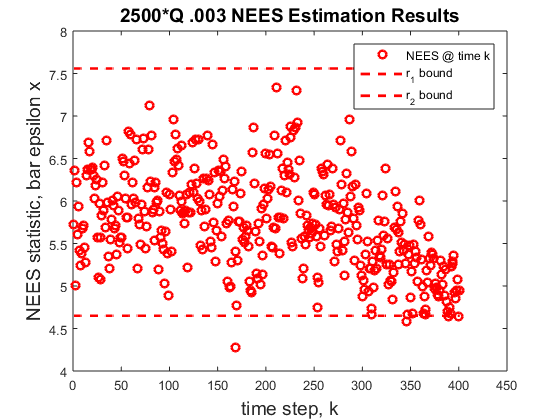
\includegraphics[width=\textwidth]{Images/QFNEES.png}
    \end{subfigure}
    \begin{subfigure}[b]{0.49\textwidth}
        \centering
        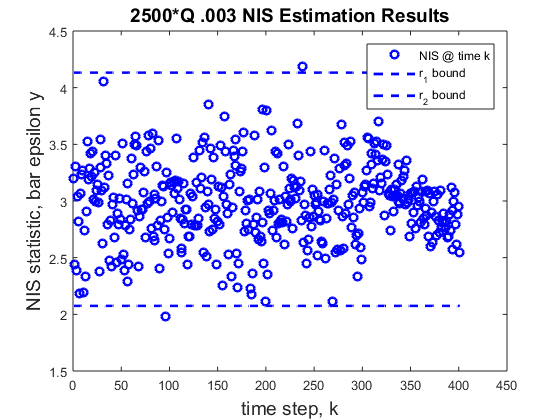
\includegraphics[width=\textwidth]{Images/QFNIS.png}
    \end{subfigure}
    \caption{NEES and NIS with 2500*Q}
    \label{nissim4}
\end{figure}


In a similar test we can evaluate system consistency when the process noise matrix Q is not fully known (which is often times the case) and is instead estimated or "guessed".  In many scenarios the process noise is the least known component of a system and is often "tuned" during simulation to verify consistency.  As previously mentioned, the NEES and NIS test are ways to determine if your Kalman Filter is finely tuned and similarly, how refined the process noise matrix is in your sytem.  To test this aspect, our team ran additional NEES and NIS simulations with steady amplification of the process noise, Q in an effort to throw our simulation out of balance.  Maintain the rigid requirements of 3 sigmas and executing 50 Monte Carlo runs, our system did not fail the NEES and NIS tests until process noise was multiplied by a factor of $> 2000$ as is seen in figure \ref{nissim4} and figure \ref{nissim5}.

\begin{figure}[h!]
    \begin{subfigure}[b]{0.49\textwidth}
        \centering
        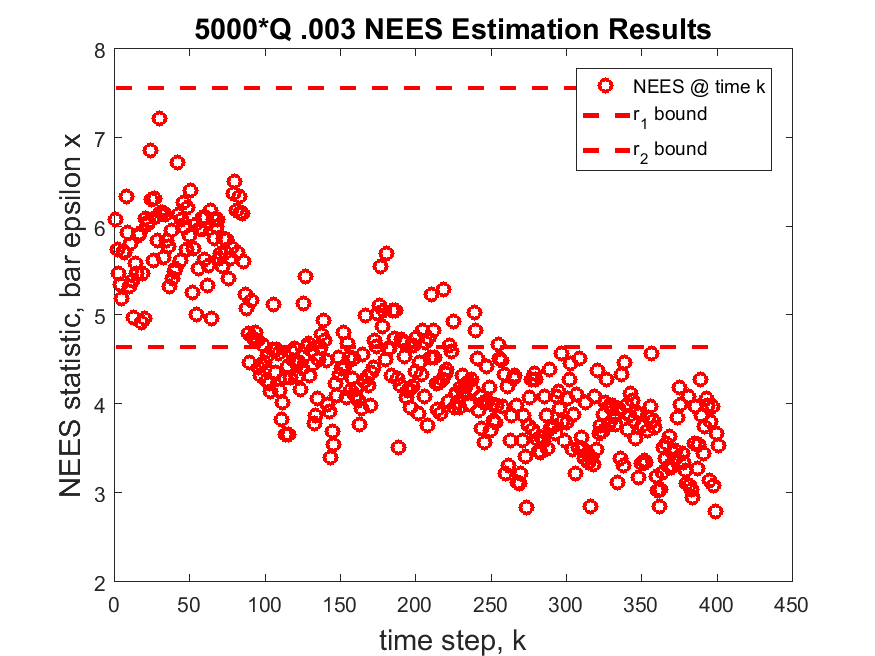
\includegraphics[width=\textwidth]{Images/5000NEES.png}
    \end{subfigure}
    \begin{subfigure}[b]{0.49\textwidth}
        \centering
        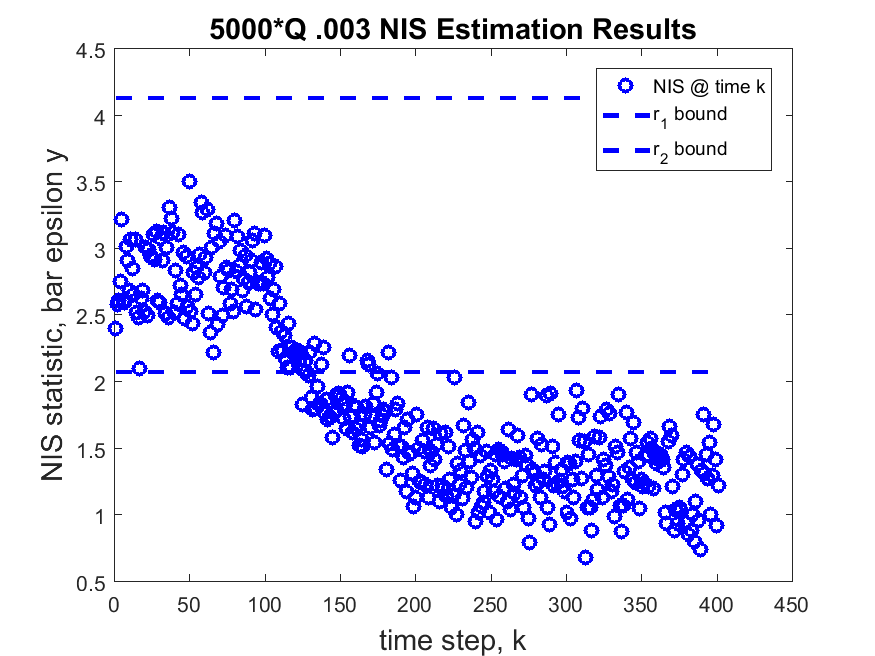
\includegraphics[width=\textwidth]{Images/5000NIS.png}
    \end{subfigure}
    \caption{NEES and NIS with 5000*Q}
    \label{nissim5}
\end{figure}
}
}
\vspace{2cm}
\section{Final Thoughts and Further Work}{
Overall, this has been an enlightening project governing state estimation in simulation of a multirotor. Several different versions of the Kalman Filter were explored and analyzed as well as related topics like system initialization and noise characterization. It has been a nice culmination of the work throughout this semester. For future and further work we would like to explore non-linear dynamics and some of the unsolved problems in terms of yaw for this project, potentially looking into the extended Kalman Filter. Thanks again and happy holidays.

\subsection{Haiku}

{
Where is the damn quad?\\
Kalman helps us estimate\\
If we code correct
}
}

\clearpage
\begin{thebibliography}{9}
    \bibitem{anderson} Anderson, B., Moore, J., \textit{Optimal Filtering.} Prentice Hall, NJ, 1979.
    \bibitem{assimakis} Assimakis, N., \textit{Information Filter and Kalman Filter Comparison:  Selection of the Faster Filter.} International Journal of Information Engineering, Vol. 2, March, 2012.
    \bibitem{bouabdallah} Bouabdallah, S., Becker, M., \textit{Towards obstacle avoidance on
    quadrotor.} International Symposium on Dynamic Problems of Mechanics, 2007.
    \bibitem{brown} Brown, R., Hwang, P., \textit{Introduction to Random Signals and Applied Kalman Filtering.} J. Wiley, NY, 2012.
    \bibitem{crassidis} Crassidis, J., \textit{Optimal Estimation of Dynamic Systems.} CRC Press, 2012.
    \bibitem{elkholy} Elkholy, H., \textit{Dynamic Modeling and Control of a Quadrotor Using Linear and Nonlinear Approaches.} American University in Cairo, 2014.
    \bibitem{mellinger} Mellinger, D., \textit{Trajectory Generation and Control for Precise Aggressive Maneuvers with Quadrotors.} International Robot Research, Apr, 2012.
    \bibitem{verhaegen}Verhaegen, M., Van Dooren, P., \textit{Numerical Aspects of Different Kalman Filter Implementations.} IEEE Transactions on Automatics Control, Vol. 10, Oct, 1986.
    \bibitem{welch} Welch, G., Bishop, G., \textit{An Introduction to the Kalman Filter.} University of North Carolina at Chapel Hill, July 2006.
    \bibitem{web}website:\texttt{https://www.researchgate.net/figure/275626071\_fig1\_Figure-1\\
    -Quadrotor-configuration}
\end{thebibliography}

\newpage
\appendix
\section*{Matlab Code}
The matlab code used is attached in the zip folder containing this project.
%\lstset{language=Matlab,%
    %basicstyle=\color{red},
%    breaklines=true,%
%    morekeywords={matlab2tikz},
%    keywordstyle=\color{blue},%
%    morekeywords=[2]{1}, keywordstyle=[2]{\color{black}},
%    identifierstyle=\color{black},%
%    stringstyle=\color{magenta},
%    commentstyle=\color{green},%
%    showstringspaces=false,%without this there will be a symbol in the places where there is a space
%    numbers=left,%
%    numberstyle={\tiny \color{black}},% size of the numbers
%    numbersep=9pt, % this defines how far the numbers are from the text
%    emph=[1]{for,end,break},emphstyle=[1]\color{red}, %some words to emphasise
%    %emph=[2]{word1,word2}, emphstyle=[2]{style},   
%    basicstyle=\small
%}
%\subsection*{One Step Kalman Filter}
%\lstinputlisting{KAL_FILT.m}
%\subsection*{One Step Fixed Gain Observer}
%\lstinputlisting{Burger_Observer.m}
%\subsection*{Full Code}
%\lstinputlisting{code.m}


\end{document}